\documentclass{article}

\usepackage{template}
\usepackage[acronym]{glossaries}
\usepackage{hyperref}

\title{Pinpoint: multi-probe trajectory planning for electrophysiology using an interactive web-based 3D environment}

% TODO LIST

% dan
% - draft figures
% - draft text (1500 word limit)
% - author list: steven (for mri alignment?), probably not yoni/josh for this simplified paper
% - video for (1) accounts, (2) automation

% kenneth
% - think about what will go on figure
% - look at draft of results
% - methods for ephys link

% three figures
% 1: overview figure
% 1a large image of pinpoint
% 1b zoom view of individual shanks
% 1c zoom view of in-plane slice
% 1d zoom view different probe options
% 1e craniotomy
% 1f surgery coordinates
% 1g accounts

% 2: coordinate spaces

% 3: rig parts and collisions
% 3a steinmetz lab well 
% 3b IBL headbar
% 3c 2-photon lens + headbar

% 4: automation
% 4a ephys link
% 4b echoing
% 4c automation

\author[1,3,*]{Daniel Birman}
\author[1]{Kenneth Yang}
% \author[3]{The International Brain Lab}
\author[1,3]{Nicholas A. Steinmetz}
\affil[1]{Department of Biological Structure, University of Washington, Seattle, WA 98195, USA}
% \affil[2]{Allen Institute, Seattle, WA 98109, USA}
\affil[3]{International Brain Laboratory, ?, ?, ?}
\affil[*]{Corresponding author: dbirman@uw.edu}

\date{\today}


% command examples
% \newcommand{\NImagesToIntroduceCategory}{5}

\begin{document}

% acronym example
% \newacronym{short}{short text}{long text}

\maketitle
% elife tools & resources paper
% We welcome the submission of Short Reports, for example reporting the results of a single set of experiments, provided the conclusion is clear and justified, and the findings are novel and judged to be of high importance. Short Reports should not usually exceed 1,500 words in the main text, excluding the Materials and Methods, References, and Figure legends, with no more than three or four main display items (figures, tables, videos). Authors have more flexibility in the format, for example with a combined Results and Discussion section.

\section{Abstract}
Targeting deep brain structures during electrophysiology experiments requires intensive training and expertise. Even with experience, the time constraints of typical experimental setups often make it difficult to know whether an electrode is placed precisely in a target location and this complexity scales with the number of simultaneous electrodes used in a recording. Existing software for trajectory planning often requires extensive programming skills to run or investment in a specific hardware setup. Here, we present \textit{Pinpoint}, open-source software that allows for interactive exploration of insertion plans for multi-probe electrophysiology. Once an insertion plan is created, Pinpoint provides easy-to-use coordinates for targeting electrodes during experiments. Pinpoint also exposes real-time visualization features to help users see their probe positions in the live brain during recordings, as well as automation to make the insertion process more efficient. Pinpoint runs in a web browser with no dependencies or installation and has a minimal learning curve. This makes Pinpoint useful not only for experiment planning, but also for exploring mouse brain anatomy and for teaching new researchers about how \textit{in vivo} experiments are performed. 

\clearpage

\linenumbers

\section{Introduction}

The availability of high-density low-cost silicon probes \citep{jun2017fully} has led to a step change in the scale \citep{steinmetz2019distributed} and ambition \citep{koch2022next} of modern neuroscience. This significant advance in hardware has not been fully matched by a similar improvement in the software interfaces used for performing experiments. Although some aspects of performing electrophysiology experiments are now possible through intuitive open-source interfaces, including data acquisition \citep{siegle2017open}; planning experiments, performing surgical targeting, and assessing probe position in real time continues to require significant expertise on the part of researchers. Experimental design should not require researchers to have expert anatomical knowledge of the entire brain, instead, experimental planning tools should provide users with easy-to-use and intuitive interfaces that guide them in designing and executing optimal probe insertion plans for their experimental goals. 

\section{Results and Discussion}

Pinpoint provides users with an interactive 3D scene in which electrophysiology trajectories can be explored within the anatomical context of the mouse brain (Fig. Xy). At the center of the 3D scene we render transparent 3D meshes for the major brain structures in the mouse Common Coordinate Framework (CCF) \citep{wang2020allen}. Individual brain regions can be highlighted through a search menu. 3D models of Neuropixels probes \citep{jun2017fully} can be added to the scene and moved through intuitive click+drag (or keyboard) interactions. Pinpoint provides feedback on the brain areas that each probe is passing through via a ``probe panel'' and an ``in-plane slice''. The view has space to render 16 probe shanks at a time, supporting either 16 individual 1-shank Neuropixels probes or four 4-shank probes. Additional features include the ability to snap probes to brain regions, design plans for craniotomy surgeries, detect collisions between probes and between probes and rig hardware, save experimental plans, and automate experiments. By running in both web browsers and as a standalone application, Pinpoint lowers the barrier to experimental planning and disconnects the need for expert anatomical knowledge of the brain from the technical skill required to perform complex simultaneous multi-probe recordings. 

\begin{figure}
\centering

\includegraphics[keepaspectratio,width=0.4\textwidth]{figures/figure-1.pdf}
\caption[mini-caption]{Title. Caption}
\label{fig:pinpoint_overview}
\end{figure}

\subsection{Planning an insertion in 3D space}

In the following sections we describe the features in Pinpoint that enable users to plan a trajectory. These steps can also be followed in online \href{https://virtualbrainlab.org/02_traj_planner/02_tp_tutorial.html}{video tutorials}. 

To target particular brain regions users can snap probes to the center of regions and then perform further manual alignment to optimize their trajectory in 3D space. By default, Pinpoint loads the top-level of the CCF hierarchy and displays these brain regions as transparent meshes. To target more specific regions or layers, users can search for these in the search bar (Figure). Clicking on a region highlights the 3D mesh in the scene using an opaque texture and pressing the ``snap'' button moves the probe tip to the center of the 3D mesh. Once the probe tip is positioned, users can use either click+drag controls with their mouse, or keyboard presses to optimize the alignment. To use the keyboard controls, users press the keys corresponding to the different axis directions: anterior-posterior: W and S, left-right A and D, dorsal-ventral: E and Q. Users can also rotate probes: pitch: R and F, yaw: 1 and 3, spin: , and . . To move the probe along its depth axis users can press Z or X. Each of these keyboard presses moves the probe tip by 10 um along that axis. Holding shift increases the step size to 100 um while holding control reduces it to 1 um. To use the click+drag controls, users click the left mouse button on the 3D model of the probe and then press any of the axis keys (e.g. W or S for anterior-posterior). Dragging the mouse along the corresponding axis will then move the probe continuously.

% stereo coordinates
After planning a recording, Pinpoint provides users with the stereotaxic coordinates and angles needed to reproduce the insertion in the live mouse brain. Pinpoint defines an insertion using the entry coordinate on the surface of the brain, defined by its (AP, ML, DV) position relative to Bregma (??). Probe angles are defined as (Pitch, Yaw, Spin), where pitch is the angle off of the horizontal plane, yaw is the rotation of the probe around the Z (up) axis, and spin is the rotation of the probe around its own axis. To perform a recording, users set up their probe according to the specified angles, zero their stereotax with the probe tip at Bregma, and move the probe to the entry coordinate. Once at the entry coordinate, the target brain area is reached by moving only along the depth axis.

\begin{figure}
\centering
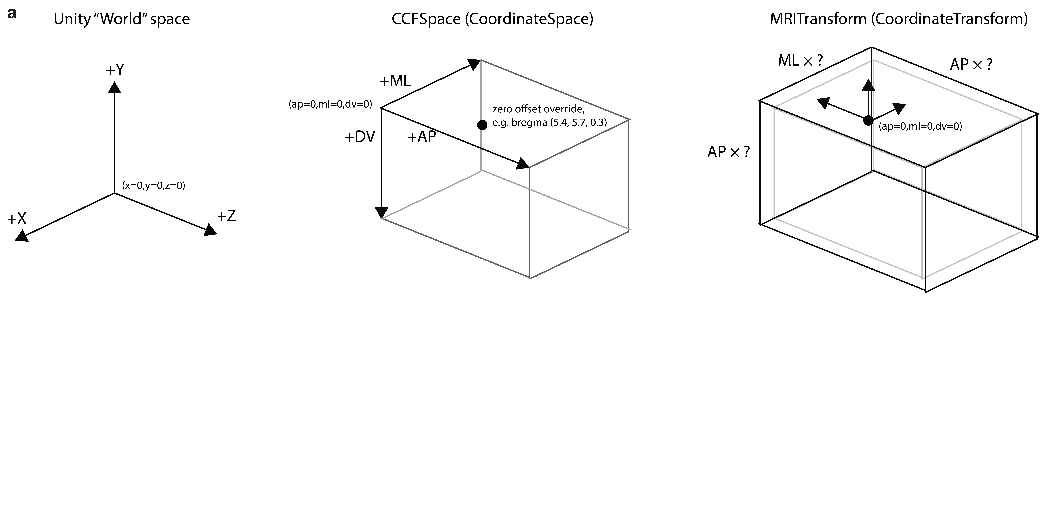
\includegraphics[keepaspectratio,width=0.4\textwidth]{figures/figure-2.pdf}
\caption[mini-caption]{Title. Caption}
\label{fig:coordinate_spaces}
\end{figure}

% coordinate spaces
When using Pinpoint, users can choose to plan their trajectories in raw CCF space or in a deformation of CCF to better match the live mouse brain. The CCF was defined using perfused brains, which are warped and stretched compared to the live brain. The transformed spaces were defined from anatomical MRI images that were aligned to the CCF, but in theory provide a better estimate of the live mouse brain depending on the age and strain. We provide a variety of transformation options as well as options to scale the transformed space according to the Bregma-Lambda distance.

\begin{figure}
\centering
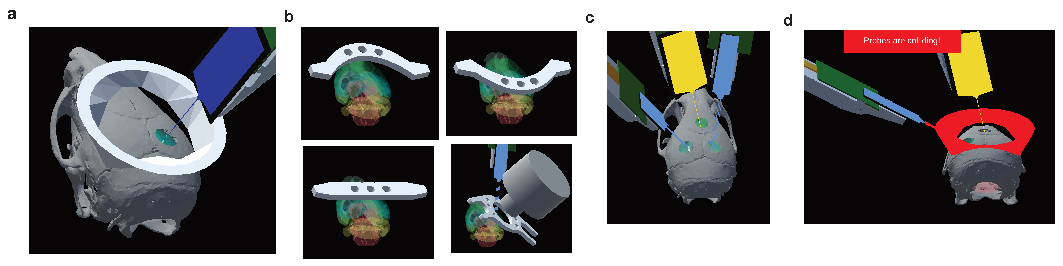
\includegraphics[keepaspectratio,width=0.4\textwidth]{figures/figure-3.pdf}
\caption[mini-caption]{Title. Caption}
\label{fig:rig_hardware}
\end{figure}

% avoiding rig hardware
The interactive 3D scene in Pinpoint provides a number of affordances that help with planning trajectories alongside complex surgical and hardware constraints. Alongside the 3D probe models, Pinpoint can display a skull model and allow users to explore possible craniotomies for surgery (Fig. Xy). Another example, simultaneous recordings with both 2-photon calcium imaging and electrophysiology probes, imaging hardware can limit the angles at which probes can be inserted.

% saving experiments

\subsection{Automation}

\begin{figure}
\centering
\includegraphics[keepaspectratio,width=0.4\textwidth]{figures/figure-4.pdf}
\caption[mini-caption]{Title. Caption}
\label{fig:automation}
\end{figure}

% live echoing
In addition to the trajectory planning features, we also designed Pinpoint to act as a link to hardware manipulators, both to show the live position of probes in the brain and to enable automated insertion of probes. In parallel to Pinpoint we have developed a Python package ``ephys-link'' that handles communication with hardware manipulators (currently, Sensapex uMP-4 and New Scale ??). Ephys-link automatically detects and communicates with connected manipulators and exposes a WebSocket connection for communicating with Pinpoint. Once connected, users have to ensure that their probe type and angles match the live probe and set a reference point so that Pinpoint can compute the relative position of the live probe in the 3D scene. After linking, probe movements are echoed in the scene allowing users to visualize their probe position live in the mouse brain. 

% automated insertions
When connected to the ephys-link package, Pinpoint can also perform some parts of the insertion process automatically. We have developed automation tools to accelerate the process of handling large numbers of probes, in particular to enable users to perform 4+ multi-probe recordings in an efficient and safe manner. To do this, we have built into Pinpoint a standard sequence for performing multi-probe insertions: first, users set up the Pinpoint scene to have the 3D models of all probes (Fig. Xy), second, they link these probes to the hardware manipulators and choose the target insertions (Fig. Xy), third, they zero all of the probes at Bregma individually, and finally, they allow the insertion sequence to run. The sequence moves probes first to their insertion coordinate, then allows the user to punch through the dura, and finally drives the probes to the appropriate depth. In the future, we hope to enable complete automation through the use of external cameras to detect probe positions, craniotomy locations, blood vessels, and probe bending during insertion. 

\section{Methods}
\subsection{Application and Code}

Pinpoint is available as a website and a standalone application. New releases can be found on the \href{https://github.com/VirtualBrainLab/Pinpoint/releases}{release page} on Github. Documentation and tutorials can be found on our \href{https://virtualbrainlab.org/02_traj_planner/01_tp_intro.html}{main website}. 

Pinpoint is developed using the Unity Real-Time Development Platform (Unity). Unity is a cross-platform game engine that supports the development of interactive 2D and 3D experiences. We use a number of specific Unity packages to support features in Pinpoint.

\begin{center}
\begin{tabular}{ |p{3cm}|p{8cm}| }
\hline
 Package & Description \\ 
 \hline
 Unity base editor 2021.3.10f1 & The main Unity editor enables the core features in Pinpoint, including the 3D scene, use of materials and shaders, the point-and-click interaction, and the user interface. \\ 
 \hline
 Addressables & Asynchronous loading of large files, such as the Common Coordinate Framework 3D models \\
 \hline
\end{tabular}
\end{center}

\subsection{Coordinate spaces and atlases}

To convert the mouse CCF \citep{wang2020allen} atlas into an anatomical MRI space we registered the CCF atlas to the 

\subsection{Contributing}

Pinpoint is an open-source project and is open to contributions from the neuroscience community. Instructions for developing and contributing to Pinpoint can be found on our \href{https://virtualbrainlab.org/02_traj_planner/05_tp_development.html}{development page}.


\subsection{Acknowledgments}

We acknowledge the generous support of the Washington Research Foundation Postdoctoral Fellowship to DB. Thank you to Kai Nylund for testing some early prototypes.

WRF
The Wellcome Trust (216324)
The Simons Foundation

\subsection{Contributions}

% Contributions go here

\printbibliography


\end{document}